\documentclass[10pt,a4paper]{article}
\usepackage[margin=0.7in]{geometry}
\usepackage{multicol}
\usepackage{amsmath}
\usepackage{tikz}
\usepackage{enumitem}
\usepackage{titlesec}
\usepackage{booktabs}
\usepackage{fontspec}

% Compact formatting
\setlength{\columnsep}{0.7cm}
\setlength{\parindent}{0pt}
\setlength{\parskip}{0.12cm}
\titlespacing{\section}{0pt}{0.4cm}{0.15cm}
\titlespacing{\subsection}{0pt}{0.25cm}{0.08cm}
\titlespacing{\subsubsection}{0pt}{0.2cm}{0.05cm}

% Custom section style
\titleformat{\section}{\large\bfseries}{}{0em}{}
\titleformat{\subsection}{\normalsize\bfseries}{}{0em}{}
\titleformat{\subsubsection}{\normalsize\bfseries\itshape}{}{0em}{}

\begin{document}

\begin{center}
{\LARGE \textbf{Macroeconomics: Key Concepts and Analysis}}\\[0.15cm]
{\normalsize \textit{Topic 8: National Income, Macroeconomic Problems, Policy, and Investment Appraisal}}\\[0.15cm]
\hrule
\end{center}
\vspace{-0.3cm}

\begin{multicols}{2}
\footnotesize

% ============================================================================
% PART 1: DEFINITIONS AND CORE CONCEPTS
% ============================================================================
\section*{1. Core Definitions and Foundational Concepts}

\subsection*{What is Macroeconomics?}
\textbf{Macroeconomics} is the branch of economics that studies the behavior and performance of the \textbf{economy as a whole}. It focuses on aggregate measures such as total output, total employment, the general price level, and the overall rate of economic growth. Unlike microeconomics (individual markets), macroeconomics deals with \textbf{aggregate variables} and the interactions between broad sectors.

\textbf{Key Macroeconomic Questions:}
\begin{itemize}[leftmargin=*,nosep]
    \item Why do some countries grow faster than others?
    \item What causes unemployment and inflation?
    \item How can government policy stabilize the economy?
    \item What determines interest rates, exchange rates, and the balance of trade?
\end{itemize}

\subsection*{GDP, GNP, and National Income}
\textbf{Gross Domestic Product (GDP):} The total \textbf{market value} of all \textbf{final} goods and services produced within a country's \textbf{geographic borders} in a given period (usually a year).

\textbf{Gross National Product (GNP):} The total market value of all final goods and services produced by a country's \textbf{residents} (citizens and firms), regardless of where production takes place.
\[
GNP = GDP + \text{Net Factor Income from Abroad (NFIA)}
\]
NFIA = Income earned by domestic residents abroad minus income earned by foreigners within the country. Example: Profit remitted by Toyota's US factory to Japan counts in Japan's GNP, US's GDP.

\textbf{Net National Product (NNP) and National Income (NI):}
\[
NNP = GNP - \text{Depreciation (Capital Consumption Allowance)}
\]
\[
NI = NNP - \text{Indirect Business Taxes} + \text{Subsidies}
\]
National Income ($Y$) can be measured via three approaches (\textbf{Circular Flow Identity}):
\begin{enumerate}[leftmargin=*,nosep]
    \item \textbf{Expenditure Approach:} $Y = C + I + G + (X - M)$
    \item \textbf{Income Approach:} $Y = \text{Wages} + \text{Rent} + \text{Interest} + \text{Profit}$
    \item \textbf{Value-Added (Product) Approach:} Sum of value added at each stage of production.
\end{enumerate}

\subsection*{Nominal GDP vs. Real GDP}
\textbf{Nominal GDP:} GDP measured at \textbf{current market prices}. It can increase due to higher production (real growth) or higher prices (inflation). $\text{Nominal GDP}_t = \sum P_t \times Q_t$.

\textbf{Real GDP:} GDP measured at \textbf{constant base-year prices}. It isolates changes in physical output, removing the effect of price changes. $\text{Real GDP}_t = \sum P_{\text{base}} \times Q_t$.

\textbf{GDP Deflator (Price Index):}
\[
GDP\ \text{Deflator} = \frac{\text{Nominal GDP}}{\text{Real GDP}} \times 100
\]
It measures the \textbf{overall price level} of all goods and services included in GDP. It is a broader measure than CPI (Consumer Price Index), which only covers consumer goods.

\subsection*{Saving, Consumption, and Investment}
\begin{itemize}[leftmargin=*,nosep]
    \item \textbf{Consumption ($C$):} Spending by households on goods and services (durables, non-durables, services). The largest component of GDP (60--70\% in developed economies).
    \item \textbf{Saving ($S$):} The part of disposable income not spent on consumption. $S = Y_d - C$. The \textbf{Marginal Propensity to Save (MPS)} is the fraction of an additional dollar of income that is saved. $MPS = \Delta S / \Delta Y$.
    \item \textbf{Investment ($I$):} Spending by firms on \textbf{capital goods} (machinery, factories, equipment), changes in \textbf{inventories}, and \textbf{residential construction}. It is a \textbf{flow} concept (adding to the \textbf{stock} of capital). Gross Investment = Net Investment + Depreciation.
\end{itemize}

\textbf{Key Relationships:}
\begin{itemize}[nosep]
    \item \textbf{Consumption Function (Keynes):} $C = a + bY_d$, where $a$ is autonomous consumption, $b$ is MPC ($0 < b < 1$).
    \item \textbf{Saving Function:} $S = -a + (1-b)Y_d = -a + MPS \cdot Y_d$.
    \item \textbf{MPC + MPS = 1.}
    \item In a closed economy with no government: $Y = C + I$ and at equilibrium, $S = I$.
\end{itemize}

% ============================================================================
% PART 2: HOW TO REMEMBER
% ============================================================================
\section*{2. Memory Triggers and Conceptual Anchors}

\begin{itemize}[leftmargin=*,nosep]
    \item \textbf{GDP vs. GNP:} ``D'' for \textbf{D}omestic (within borders, no matter who produces). ``N'' for \textbf{N}ational (citizens, no matter where). Mnemonic: \textbf{GDP = Geography; GNP = Nationality (Passport).}
    \item \textbf{Nominal vs. Real:} \textbf{N}ominal = \textbf{N}ow prices (current, inflated). \textbf{R}eal = \textbf{R}eal quantity (base-year prices, apples-to-apples comparison across time).
    \item \textbf{GDP Deflator = ``Inflation Remover'':} Deflator $\uparrow$ means prices have risen. To convert Nominal to Real: $\text{Real} = \text{Nominal} / (\text{Deflator} / 100)$.
    \item \textbf{The Circular Flow:} Households supply labor $\to$ Firms pay wages $\to$ Households consume $\to$ Firms produce. Income = Expenditure = Output. \textbf{``One person's spending is another person's income.''}
    \item \textbf{Consumption and Saving:} MPC = ``If I get an extra dollar, how much of it do I spend?'' MPS = ``...how much do I save?'' They must sum to 1.
    \item \textbf{Unemployment Types:}
    \begin{itemize}[nosep]
        \item \textbf{Frictional:} ``Between jobs'' -- searching, transitioning. Normal, healthy.
        \item \textbf{Structural:} ``Skills mismatch'' -- your job skills are obsolete (e.g., coal miner in a green economy). Requires retraining.
        \item \textbf{Cyclical:} ``Because the economy is bad'' -- due to recession, insufficient aggregate demand. Policy can fix this.
    \end{itemize}
    \item \textbf{Inflation = Too Much Money Chasing Too Few Goods:} Demand-pull (economy overheated) vs. Cost-push (input prices rise, e.g., oil shock).
    \item \textbf{Fiscal vs. Monetary Policy:} \textbf{Fiscal} = Government (Congress, Treasury) -- taxes and spending. \textbf{Monetary} = Central Bank (Fed) -- interest rates, money supply. Mnemonic: ``\textbf{F}iscal = \textbf{F}ederal budget; \textbf{M}onetary = \textbf{M}oney supply.''
    \item \textbf{NPV, IRR, Payback -- Investment Decision Mnemonics:}
    \begin{itemize}[nosep]
        \item \textbf{NPV:} ``\textbf{N}et \textbf{P}resent \textbf{V}alue'' -- accept if positive ($NPV > 0$).
        \item \textbf{IRR:} ``\textbf{I}nternal \textbf{R}ate of \textbf{R}eturn'' -- accept if IRR > cost of capital.
        \item \textbf{Payback Period:} ``How fast do I get my money back?'' Shorter is better.
    \end{itemize}
\end{itemize}

% ============================================================================
% PART 3: MATHEMATICAL FRAMEWORK
% ============================================================================
\section*{3. Mathematical Formulation and Models}

\subsection*{National Income Identity (Expenditure)}
\[
Y = C + I + G + NX
\]
Where $NX = X - M$ (Net Exports). In a closed economy without government: $Y = C + I$.

\subsection*{Equilibrium in the Keynesian Cross Model}
Aggregate Expenditure ($AE$) = $C + I + G + NX$. Equilibrium: $Y = AE$.
With $C = a + bY_d$, $Y_d = Y - T$ (disposable income, $T$ = taxes net of transfers):
\[
Y = a + b(Y - T) + I + G + NX
\]
Solving for $Y$:
\[
Y = \frac{1}{1-b} \left( a - bT + I + G + NX \right)
\]
The \textbf{multiplier} $k = \frac{1}{1-b} = \frac{1}{MPS}$. A \$1 change in autonomous spending changes equilibrium output by \$k.

\subsection*{Inflation Rate}
\[
\pi_t = \frac{P_t - P_{t-1}}{P_{t-1}} \times 100
\]
Where $P_t$ is the price level (CPI or GDP Deflator) in period $t$.

\subsection*{Unemployment Rate}
\[
u = \frac{\text{Unemployed}}{\text{Labor Force}} \times 100
\]
Labor Force = Employed + Unemployed (actively seeking work). Note: Discouraged workers (not seeking) are not counted in the labor force.

\subsection*{Okun's Law (Relationship: Output and Unemployment)}
A 1 percentage point increase in cyclical unemployment is associated with approximately a 2\% decline in output relative to potential GDP (varies by country/time). $\frac{Y - Y^*}{Y^*} \approx -2 (u - u^*)$.

\subsection*{Phillips Curve (Short-Run Trade-off)}
\[
\pi = \pi^e - \beta (u - u^*) + \nu
\]
Where $\pi$ is actual inflation, $\pi^e$ is expected inflation, $u^*$ is natural rate of unemployment, $\nu$ is a supply shock. In the short run, there is a trade-off between inflation and unemployment. In the long run, the curve is vertical at the natural rate ($u = u^*$).

\subsection*{Investment Decision Rules}
\textbf{Net Present Value (NPV):}
\[
NPV = \sum_{t=0}^{n} \frac{CF_t}{(1 + r)^t}
\]
Where $CF_t$ = net cash flow in year $t$, $r$ = discount rate (cost of capital), $n$ = project life. \textbf{Decision:} Accept if $NPV > 0$.

\textbf{Internal Rate of Return (IRR):} The discount rate $r^*$ such that $NPV = 0$.
\[
0 = \sum_{t=0}^{n} \frac{CF_t}{(1 + r^*)^t}
\]
\textbf{Decision:} Accept if $IRR > r$ (cost of capital).

\textbf{Payback Period:} The time (usually years) required for cumulative net cash flows to equal the initial investment. Simpler but ignores time value of money and cash flows beyond payback.

\textbf{Cost-Benefit Analysis (CBA):} Systematic process of comparing total social benefits against total social costs of a project or policy, often including non-market valuation (environmental, health). Converts all impacts to monetary terms where possible. Benefit-Cost Ratio: $BCR = \frac{\sum B_t/(1+r)^t}{\sum C_t/(1+r)^t}$. Accept if $BCR > 1$.

% ============================================================================
% PART 4: GRAPHICAL ANALYSIS
% ============================================================================
\section*{4. Graphical Illustrations}

\subsection*{Circular Flow of Income (Two-Sector)}
\begin{center}
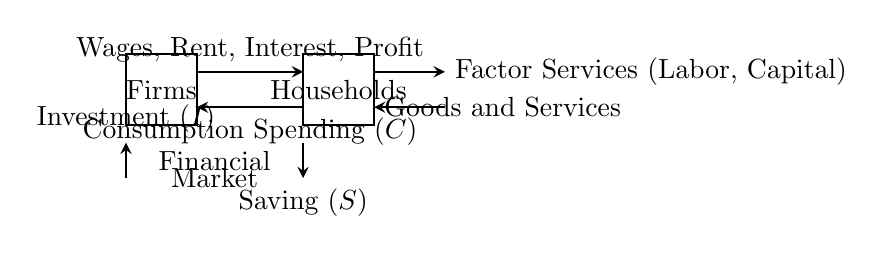
\begin{tikzpicture}[scale=0.45, thick, >=stealth]
    % Firms
    \draw (0,2) rectangle (2,4) node[midway] {Firms};
    % Households
    \draw (5,2) rectangle (7,4) node[midway] {Households};
    % Flows
    \draw[->] (2,3.5) -- (5,3.5) node[midway, above] {Wages, Rent, Interest, Profit};
    \draw[->] (5,2.5) -- (2,2.5) node[midway, below] {Consumption Spending ($C$)};
    \draw[->] (7,3.5) -- (9,3.5) node[right] {Factor Services (Labor, Capital)};
    \draw[->] (9,2.5) -- (7,2.5) node[right] {Goods and Services};
    \draw[->] (5,1.5) -- (5,0.5) node[below] {Saving ($S$)};
    \draw[->] (0,0.5) -- (0,1.5) node[above] {Investment ($I$)};
    \node at (2.5,1) {Financial};
    \node at (2.5,0.5) {Market};
\end{tikzpicture}
\end{center}
\textit{Inner loop: Real flows (factors, goods). Outer loop: Money flows (income, spending). Leakage: Saving. Injection: Investment. In equilibrium: $S = I$.}

\subsection*{Keynesian Cross: Equilibrium Output}
\begin{center}
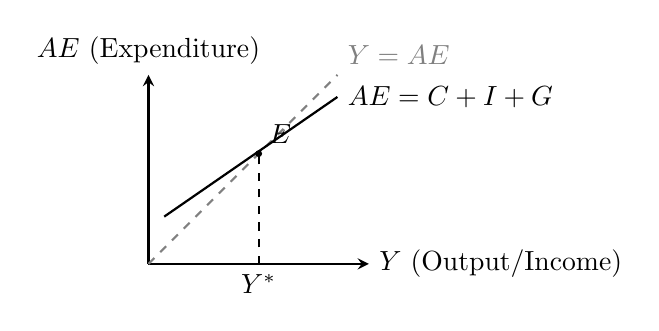
\begin{tikzpicture}[scale=0.4, thick, >=stealth]
    \draw[->] (0,0) -- (7,0) node[right] {$Y$ (Output/Income)};
    \draw[->] (0,0) -- (0,6) node[above] {$AE$ (Expenditure)};
    % 45-degree line
    \draw[thick, dashed, gray] (0,0) -- (6,6) node[above right] {$Y=AE$};
    % AE curve
    \draw[thick] (0.5,1.5) -- (6,5.3) node[right] {$AE = C + I + G$};
    % Equilibrium
    \filldraw (3.5,3.5) circle (2pt) node[above right] {$E$};
    \draw[dashed] (3.5,0) node[below] {$Y^*$} -- (3.5,3.5);
\end{tikzpicture}
\end{center}
\textit{Equilibrium where $AE$ line intersects the 45-degree line ($Y=AE$). If $Y < Y^*$, inventories fall unexpectedly, firms increase production. The multiplier amplifies changes in autonomous spending.}

\subsection*{Phillips Curve (Short-Run vs. Long-Run)}
\begin{center}
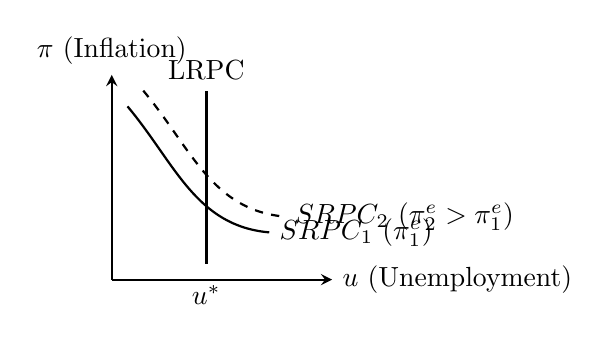
\begin{tikzpicture}[scale=0.4, thick, >=stealth]
    \draw[->] (0,0) -- (7,0) node[right] {$u$ (Unemployment)};
    \draw[->] (0,0) -- (0,6.5) node[above] {$\pi$ (Inflation)};
    % LRPC (vertical)
    \draw[very thick] (3,0.5) -- (3,6) node[above] {LRPC};
    \node at (3,-0.5) {$u^*$};
    % SRPC curves
    \draw[thick] (0.5,5.5) to[out=310, in=175] (5,1.5) node[right] {$SRPC_1$ ($\pi^e_1$)};
    \draw[thick, dashed] (1,6) to[out=310, in=175] (5.5,2) node[right] {$SRPC_2$ ($\pi^e_2 > \pi^e_1$)};
\end{tikzpicture}
\end{center}
\textit{Short-run Phillips Curve (SRPC) slopes down: lower unemployment temporarily achievable with higher inflation. Long-run Phillips Curve (LRPC) is vertical at the Natural Rate of Unemployment ($u^*$): no long-run trade-off.}

% ============================================================================
% PART 5: FISCAL AND MONETARY POLICY
% ============================================================================
\section*{5. Macroeconomic Policy}

\subsection*{Fiscal Policy}
Conducted by the \textbf{government} (Treasury/Finance Ministry). Uses \textbf{government spending ($G$)} and \textbf{taxation ($T$)} to influence aggregate demand.
\begin{itemize}[leftmargin=*,nosep]
    \item \textbf{Expansionary:} Increase $G$ or decrease $T$ $\to$ boosts AD (shifts AE up/IS right). Used during recession. Financed by borrowing (deficit spending).
    \item \textbf{Contractionary:} Decrease $G$ or increase $T$ $\to$ reduces AD. Used to cool overheating economy, combat inflation.
    \item \textbf{Automatic Stabilizers:} Built-in features that automatically adjust: progressive taxes (revenues fall in recession), unemployment benefits (spending rises). No new legislation required.
    \item \textbf{Limitations:} \textbf{Crowding out} -- government borrowing raises interest rates, reducing private investment. \textbf{Time lags} -- recognition, implementation, and impact lags. \textbf{Ricardian equivalence} -- consumers save tax cuts anticipating future tax hikes, neutralizing fiscal stimulus.
\end{itemize}

\subsection*{Monetary Policy}
Conducted by the \textbf{Central Bank} (e.g., Federal Reserve, ECB). Manages \textbf{money supply} and \textbf{interest rates} to achieve price stability, full employment, and economic growth.
\begin{itemize}[leftmargin=*,nosep]
    \item \textbf{Tools:}
    \begin{enumerate}[nosep]
        \item \textbf{Policy Interest Rate (e.g., Federal Funds Rate):} Lower rate $\to$ cheaper borrowing $\to$ stimulates investment and consumption $\to$ AD shifts right. Higher rate to cool economy.
        \item \textbf{Open Market Operations (OMOs):} Buying government bonds injects money into banking system (expansionary). Selling bonds withdraws money (contractionary).
        \item \textbf{Reserve Requirements:} Lower required reserve ratio allows banks to lend more. Rarely changed.
        \item \textbf{Quantitative Easing (QE):} Central bank purchases long-term securities to lower long-term rates when short-term rates near zero. Used extensively post-2008 and COVID-19.
    \end{enumerate}
    \item \textbf{Transmission Mechanism:} Policy rate $\downarrow$ $\to$ market rates $\downarrow$ $\to$ borrowing $\uparrow$ $\to$ $C$ and $I$ $\uparrow$ $\to$ AD $\uparrow$ $\to$ Output $\uparrow$, Unemployment $\downarrow$.
    \item \textbf{Inflation Targeting:} Many central banks target ~2\% inflation. If inflation exceeds target, they raise rates.
    \item \textbf{Limitations:} \textbf{Liquidity trap} -- interest rates are near zero, monetary policy ineffective (Keynesian). \textbf{Long and variable lags} (Milton Friedman).
\end{itemize}

\subsection*{Policy Mix}
Fiscal and monetary policies can work together or at cross-purposes. Example: 2008--2009 Global Financial Crisis saw coordinated expansionary fiscal (stimulus packages) and monetary (near-zero rates, QE) policy globally.

\columnbreak

% ============================================================================
% PART 6: EXTENSIVE CASE STUDIES
% ============================================================================
\section*{6. Comprehensive Case Studies}

\subsection*{Case Study 1: The Great Recession (2008--2009) and the Global Policy Response}

\textbf{Background:} The subprime mortgage crisis in the US triggered a global financial meltdown. Banks collapsed (Lehman Brothers, Sept 2008), credit markets froze, and aggregate demand plummeted. The world entered the deepest recession since the 1930s.

\textbf{Macroeconomic Impact:}
\begin{itemize}[leftmargin=*,nosep]
    \item \textbf{US GDP:} Fell by 4.3\% from peak (Dec 2007) to trough (June 2009).
    \item \textbf{Unemployment:} US unemployment rate doubled from 5.0\% (Dec 2007) to 10.0\% (Oct 2009). Cyclical unemployment surged.
    \item \textbf{Inflation:} Plummeted; fears of deflation emerged (CPI briefly negative in 2009).
    \item \textbf{Global Spillover:} World trade collapsed by over 20\%. Export-dependent economies (Germany, Japan, China) severely hit. GDP contracted globally in 2009 -- the first global GDP decline since WWII.
\end{itemize}

\textbf{Policy Response: Unprecedented Monetary and Fiscal Expansion.}

\textit{1. Monetary Policy (Federal Reserve):}
\begin{itemize}[leftmargin=*,nosep]
    \item \textbf{Interest Rate Cuts:} Fed cut Federal Funds Rate from 5.25\% (Aug 2007) to 0--0.25\% (Dec 2008). Effectively hit the \textbf{zero lower bound}.
    \item \textbf{Quantitative Easing (QE1):} With rates at zero, the Fed launched massive asset purchases. Between 2008 and 2014, the Fed's balance sheet expanded from \$900 billion to over \$4.5 trillion. Purchased mortgage-backed securities (MBS) and Treasury bonds to lower long-term rates, support housing market, and inject liquidity.
    \item \textbf{Credit Facilities:} Created special lending facilities to unfreeze commercial paper, money market, and corporate bond markets.
    \item \textbf{Effectiveness:} Prevented a complete financial meltdown. Lowered long-term mortgage rates to historical lows, supporting a housing recovery. Critics argued QE contributed to asset price bubbles and wealth inequality (wealth effect benefited asset holders).
\end{itemize}

\textit{2. Fiscal Policy (US Government):}
\begin{itemize}[leftmargin=*,nosep]
    \item \textbf{Economic Stimulus Act (2008):} \$152 billion in tax rebates. Modest impact.
    \item \textbf{American Recovery and Reinvestment Act (ARRA, 2009):} \$787 billion (later revised to \$831 billion). Largest fiscal stimulus in US history at the time. Comprised:
    \begin{itemize}[nosep]
        \item \textbf{Tax cuts (\$288B):} Personal and business tax reductions.
        \item \textbf{Spending (\$499B):} Infrastructure, education, healthcare, renewable energy, aid to states.
    \end{itemize}
    \item \textbf{Automatic Stabilizers:} Unemployment insurance extensions, food stamps (SNAP) expanded automatically, providing significant income support without new legislation.
\end{itemize}

\textbf{Analysis Using Keynesian Cross Multiplier:}
Assume MPC ($b$) = 0.6. Multiplier $k = 1/(1-0.6) = 2.5$. A \$800B fiscal stimulus would theoretically boost GDP by up to \$2,000B (if no crowding out). In reality, the multiplier was likely smaller (0.5--1.5) due to:
\begin{itemize}[nosep]
    \item \textbf{Crowding out:} Some private investment displaced (though limited at zero rates).
    \item \textbf{Imports:} Part of spending leaked abroad (open-economy multiplier smaller).
    \item \textbf{Ricardian effects:} Households saved part of tax cuts.
    \item \textbf{Uncertainty:} Deep uncertainty reduced MPC (precautionary saving rose).
\end{itemize}
Nevertheless, most economists (CBO, IMF estimates) conclude the ARRA saved/created 2--3 million jobs and prevented a much deeper recession.

\textbf{NPV of Bailouts vs. Fiscal Stimulus:}
TARP (Troubled Asset Relief Program, 2008) to bail out banks: \$700B authorized. Surprisingly, the government \textbf{earned a positive return} on bank bailouts (\~ +{\$}20B) because banks repaid with interest. CBA showed fiscal cost was minimal. NPV of auto bailout (GM, Chrysler) was arguably positive due to saved jobs and supply chains versus long-run cost.

\textbf{Global Dimensions:}
\begin{itemize}[leftmargin=*,nosep]
    \item \textbf{China:} Massive \$586B fiscal stimulus (2008--2010), mostly infrastructure investment. GDP growth remained > 8\%, preventing global depression.
    \item \textbf{Europe:} ECB cut rates but was slower. Sovereign debt crisis (Greece, 2010) forced \textbf{austerity} (contractionary fiscal policy) in the periphery, prolonging recession. Contrast with US/China expansion.
\end{itemize}

\textbf{Economic Lessons:}
\begin{enumerate}[leftmargin=*,nosep]
    \item \textbf{Zero lower bound} constrains conventional monetary policy; unconventional tools (QE) are essential but have side effects.
    \item \textbf{Fiscal policy} is a critical complement when monetary policy is exhausted.
    \item \textbf{Coordination} matters: simultaneous global fiscal expansion was more effective than any country acting alone (positive spillovers via trade).
    \item \textbf{Political economy:} Austerity during a liquidity trap is self-defeating; it deepens recession and increases debt/GDP ratio (as GDP denominator shrinks).
    \item \textbf{Investment decisions} during crisis must consider extreme uncertainty: NPV and IRR calculations fail if future cash flows are radically uncertain. Firms delayed investment despite low rates (``wait and see'' option value).
\end{enumerate}

\subsection*{Case Study 2: The Post-COVID Inflation Surge (2021--2023) and the Return of Monetary Tightening}

\textbf{Background:} After COVID-19 hit in 2020, governments and central banks unleashed an even larger stimulus than 2008. As the economy reopened, demand surged but supply chains were broken, leading to the highest inflation in 40 years.

\textbf{The Shock and Policy:}
\begin{itemize}[leftmargin=*,nosep]
    \item \textbf{Fiscal Stimulus:} US: \$2.2T CARES Act (2020), \$900B relief (Dec 2020), \$1.9T American Rescue Plan (March 2021). Total \~ \$5T, \~ 25\% of GDP.
    \item \textbf{Monetary Easing:} Fed cut rates to 0\%, resumed massive QE (\$120B/month purchases). ECB, BoJ, BoE similar.
    \item \textbf{Direct Transfers:} Unprecedented direct checks to households (\$1,200 + \$600 + \$1,400 per adult) boosted \textbf{disposable income} even as GDP fell temporarily. \textbf{Personal saving rate} spiked to 33\% (April 2020).
\end{itemize}

\textbf{Inflationary Mechanism:}
As vaccines rolled out (2021), pent-up demand exploded. But supply couldn't respond:
\begin{itemize}[leftmargin=*,nosep]
    \item \textbf{Goods demand surge:} Consumers shifted from services (travel, dining) to goods (electronics, furniture, home improvement).
    \item \textbf{Supply chain bottlenecks:} Port congestion (LA/Long Beach), semiconductor shortage (Case Study in Topic 2), labor shortages (``Great Resignation''), shipping container costs up 500\%.
    \item \textbf{Energy price spike:} Russia-Ukraine war (Feb 2022) sent oil and natural gas prices soaring (cost-push shock).
    \item \textbf{Inflation:} US CPI inflation hit 9.1\% (June 2022), UK > 11\%, Eurozone > 10\%. Far above 2\% targets.
\end{itemize}

\textbf{Monetary Policy Reversal (2022--2023):}
Central banks pivoted aggressively from easing to tightening:
\begin{itemize}[leftmargin=*,nosep]
    \item \textbf{Fed:} Raised rates from 0.25\% to 5.50\% (March 2022--July 2023) -- fastest tightening in 40 years. Began Quantitative Tightening (QT) -- shrinking balance sheet.
    \item \textbf{Transmission:} Mortgage rates jumped from 3\% to 7\%+. Housing market cooled. Business investment slowed.
    \item \textbf{Goal:} Reduce aggregate demand to bring it in line with constrained supply, cooling inflation without causing deep recession (``soft landing'').
\end{itemize}

\textbf{Evaluation of Policy -- The Soft Landing Debate:}
By mid-2024, inflation had fallen to \~ 3\% without a large rise in unemployment (remained below 4\%). This ``immaculate disinflation'' surprised many economists. Possible reasons:
\begin{enumerate}[leftmargin=*,nosep]
    \item \textbf{Supply recovery:} Bottlenecks eased; labor force participation recovered.
    \item \textbf{Well-anchored expectations:} Despite high inflation, long-term inflation expectations remained near 2\%, so \textbf{Phillips Curve} remained flat (inflation fell without requiring large unemployment increase).
    \item \textbf{Lags:} Full effect of rate hikes may still be in pipeline; recession risk not eliminated.
    \item \textbf{Fiscal contraction:} Pandemic stimulus expired, acting as automatic fiscal tightening.
\end{enumerate}

\textbf{Investment Decisions in High-Inflation Environment:}
Firms evaluating projects in 2022--2023 faced:
\begin{itemize}[leftmargin=*,nosep]
    \item \textbf{Higher discount rate ($r$):} As central bank rates rose, cost of capital ($r$) increased, reducing \textbf{NPV} of long-term projects. Green energy capital-intensive projects (wind, solar) were particularly sensitive to higher rates.
    \item \textbf{Inflation in cash flows:} Nominal revenues rose with inflation, but real costs uncertain. Distinction between real and nominal NPV became critical.
    \item \textbf{Uncertainty:} High inflation volatility made forecasting future cash flows more difficult, increasing the ``option value of waiting'' and delaying irreversible investment.
    \item \textbf{Payback period became more popular:} In uncertain times, firms favored projects with faster payback to reduce risk exposure.
\end{itemize}
\textit{Example NPV Shift:} A \$100M renewable project with \$10M annual real cash flow for 20 years. At $r = 0.04$ (real): $NPV \approx -\$100M + \$135.9M = +\$35.9M$ (Accept). At $r = 0.08$ (real, after rate hikes): $NPV = -\$100M + \$98.2M = -\$1.8M$ (Reject). Monetary tightening directly kills marginal projects.

\textbf{Economic Lessons:}
\begin{enumerate}[leftmargin=*,nosep]
    \item \textbf{Inflation} can emerge from a combination of demand-pull (massive fiscal stimulus) and cost-push (supply chain, energy) shocks.
    \item \textbf{Monetary policy} operates with lags; central banks risk over-tightening if they don't account for them.
    \item \textbf{Real vs. Nominal} distinctions are crucial for investment evaluation under changing inflation.
    \item \textbf{Fiscal-monetary interaction:} Generous fiscal transfers during supply constraints contributed to inflation, creating a policy dilemma: support citizens vs. control inflation.
    \item \textbf{The Phillips curve} is not stable; it depends on expectations, supply conditions, and credibility of central banks.
\end{enumerate}

% ============================================================================
% PART 7: EXAM QUESTIONS
% ============================================================================
\section*{7. Exam Questions \& Model Answers}

\subsection*{Question 1: National Income Calculation}
\textbf{Given the following data for a closed economy (in \$ billions): $C = 200 + 0.75Y_d$, $I = 300$, $G = 400$, $T = 200$ (lump-sum tax).}
\textbf{(a) Find equilibrium GDP.}
\textbf{(b) Calculate the government spending multiplier.}
\textbf{(c) If potential GDP is 2,800, what change in $G$ is needed to close the output gap?}
\textbf{(d) If the government simultaneously increases $G$ by 50 and $T$ by 50, what happens to equilibrium GDP? (Balanced Budget Multiplier)}

\vspace{0.05cm}
\textbf{Solution:}
\vspace{0.05cm}
\textbf{(a)} $Y_d = Y - T = Y - 200$. $AE = 200 + 0.75(Y-200) + 300 + 400 = 200 + 0.75Y - 150 + 700 = 750 + 0.75Y$. Set $Y = AE$: $Y = 750 + 0.75Y \Rightarrow 0.25Y = 750 \Rightarrow \mathbf{Y^* = 3000}$.

\textbf{(b)} Multiplier $k = 1/(1-0.75) = 1/0.25 = \mathbf{4}$.

\textbf{(c)} Output gap = $2800 - 3000 = -200$ (recessionary gap, though note 3000 > 2800, i.e., economy is above potential, i.e., inflationary gap). If potential = 2800, and current = 3000, gap = +200. To close, need $\Delta Y = -200$. $\Delta G = \Delta Y / k = -200 / 4 = \mathbf{-50}$. Reduce $G$ by 50.

\textbf{(d)} Balanced budget multiplier: $\Delta G = \Delta T = 50$. Effect: $\Delta Y = k \cdot \Delta G + k_T \cdot \Delta T$, where $k_T = -b/(1-b) = -0.75/0.25 = -3$. $\Delta Y = 4(50) + (-3)(50) = 200 - 150 = +50$.
The \textbf{Balanced Budget Multiplier = 1}: equal increase in $G$ and $T$ raises Y exactly by the amount of the increase. (Here, $1/(1-b) + (-b/(1-b)) = (1-b)/(1-b) = 1$).

\vspace{0.2cm}

\subsection*{Question 2: Real vs. Nominal GDP and Deflator}
\textbf{An economy produces only apples and oranges. Data: Base Year 2020.}

\begin{center}
\begin{tabular}{@{}l|cc|cc@{}}
\toprule
& \multicolumn{2}{c|}{\textbf{2020}} & \multicolumn{2}{c}{\textbf{2023}} \\
& Qty & Price & Qty & Price \\
\midrule
Apples & 100 & \$2 & 120 & \$3 \\
Oranges & 50 & \$4 & 60 & \$5 \\
\bottomrule
\end{tabular}
\end{center}

\textbf{(a) Calculate Nominal GDP in 2020 and 2023.}
\textbf{(b) Calculate Real GDP in 2023 at 2020 prices.}
\textbf{(c) Calculate the GDP Deflator for 2023.}
\textbf{(d) What is the growth rate of real GDP from 2020 to 2023?}

\vspace{0.05cm}
\textbf{Solution:}
\vspace{0.05cm}
\textbf{(a)} Nominal 2020 = $100(2) + 50(4) = 200 + 200 = \mathbf{400}$. Nominal 2023 = $120(3) + 60(5) = 360 + 300 = \mathbf{660}$.

\textbf{(b)} Real 2023 (at 2020 prices) = $120(2) + 60(4) = 240 + 240 = \mathbf{480}$.

\textbf{(c)} Deflator 2023 = $(660/480) \times 100 = \mathbf{137.5}$.

\textbf{(d)} Real GDP 2020 = Nominal 2020 = 400 (base year). Real growth = $(480 - 400) / 400 \times 100 = \mathbf{20\%}$. (Nominal growth was 65\%, but much was inflation.)

\vspace{0.2cm}

\subsection*{Question 3: Investment Appraisal}
\textbf{A project requires initial investment of \$500,000. Expected net cash flows: Year 1: \$150,000; Year 2: \$200,000; Year 3: \$250,000; Year 4: \$100,000. Discount rate = 10\%.}
\textbf{(a) Calculate NPV. Should the project be accepted?}
\textbf{(b) Calculate the payback period.}
\textbf{(c) If the discount rate rises to 15\%, recalculate NPV. Explain the change.}

\vspace{0.05cm}
\textbf{Solution:}
\vspace{0.05cm}
\textbf{(a)} 
$NPV = -500,000 + \frac{150,000}{1.1} + \frac{200,000}{1.1^2} + \frac{250,000}{1.1^3} + \frac{100,000}{1.1^4}$
$= -500,000 + 136,363.6 + 165,289.3 + 187,828.7 + 68,301.3$
$= -500,000 + 557,782.9 = \mathbf{+\$57,783}$. Since $NPV > 0$, \textbf{accept}.

\textbf{(b)} Cumulative cash flows: Y1: \$150,000; Y2: \$350,000; Y3: \$600,000. Initial investment \$500,000 recovered between Y2 and Y3. Fraction of Y3 needed: $(500,000 - 350,000) / 250,000 = 0.6$. Payback = \textbf{2.6 years}.

\textbf{(c)} At 15\%:
$NPV = -500,000 + 130,434.8 + 151,228.7 + 164,379.1 + 57,175.3 = -500,000 + 503,217.9 = +\$3,218$ (still positive, just barely). Higher discount rate reduces PV of distant cash flows, reducing NPV. If $r$ rises enough, NPV turns negative $\to$ reject project.

\vspace{0.2cm}

\subsection*{Question 4: Policy Analysis}
\textbf{Explain, using AD-AS or IS-LM logic, why a central bank would raise interest rates in response to high inflation. What are the risks?}

\vspace{0.05cm}
\textbf{Answer:} High inflation indicates aggregate demand exceeds aggregate supply (or supply has contracted). Raising the policy interest rate makes borrowing more expensive, reducing consumption (durables, housing) and business investment. This shifts the AD curve leftward (or shifts LM up/left), reducing output and thus reducing inflationary pressure. The \textbf{risk} is that monetary policy operates with ``long and variable lags'' (Friedman). If the central bank tightens too aggressively or late, it may: (1) overshoot and cause a recession (AD falls too much below potential), leading to unemployment; (2) fail to anchor expectations, causing a wage-price spiral; (3) trigger a financial crisis if highly leveraged sectors (real estate, banks) cannot handle higher rates; (4) exacerbate fiscal sustainability issues by raising government borrowing costs. A ``soft landing'' (reducing inflation without recession) is the goal, but historically difficult.

\end{multicols}

% ============================================================================
% SUMMARY TABLE
% ============================================================================
\vspace{0.3cm}
\begin{center}
\fbox{\begin{minipage}{0.9\textwidth}
\footnotesize
\textbf{Summary Cheat Sheet: Macroeconomics}
\begin{center}
\begin{tabular}{@{}p{3cm}p{2.5cm}p{3.5cm}@{}}
\toprule
\textbf{Concept} & \textbf{Formula/Identity} & \textbf{Key Insight} \\
\midrule
GDP (Expenditure) & $Y = C + I + G + NX$ & Total spending = Total output \\
GNP & $GNP = GDP + NFIA$ & Based on residency, not geography \\
Real GDP & $\sum P_{\text{base}} Q_t$ & Removes inflation; measures true growth \\
GDP Deflator & $\frac{\text{Nominal GDP}}{\text{Real GDP}} \times 100$ & Broadest price index \\
Consumption Function & $C = a + bY_d$ & MPC ($b$) + MPS = 1 \\
Multiplier & $k = 1/(1-b)$ & Amplifies autonomous spending changes \\
Unemployment Rate & $u = \frac{U}{LF} \times 100$ & Excludes discouraged workers \\
Inflation Rate & $\pi = \frac{P_t - P_{t-1}}{P_{t-1}} \times 100$ & \% change in price level \\
NPV & $NPV = \sum CF_t / (1+r)^t$ & Accept if $NPV > 0$ \\
IRR & $NPV = 0 \to r^*$ & Accept if $IRR > \text{cost of capital}$ \\
Fiscal Policy & $G$ and $T$ & Government spending \& taxation \\
Monetary Policy & Interest rates, money supply & Central bank manages demand \\
\bottomrule
\end{tabular}
\end{center}

\vspace{0.1cm}
\textbf{Quick Policy Reference:}
\begin{itemize}[leftmargin=*,nosep]
    \item \textbf{Recession} $\to$ Expansionary: $\uparrow G$, $\downarrow T$, $\downarrow r$, QE.
    \item \textbf{Inflation} $\to$ Contractionary: $\downarrow G$, $\uparrow T$, $\uparrow r$, QT.
    \item \textbf{Liquidity Trap} $\to$ Monetary policy ineffective; rely on fiscal policy.
    \item \textbf{NPV Rule:} Positive NPV $\to$ Accept project; IRR > Hurdle Rate $\to$ Accept.
\end{itemize}
\end{minipage}}
\end{center}

\end{document}